\chapter{Hydrodynamics Units}
\label{Chp:Hydrodynamics Unit}

The \unit{Hydro} unit solves Euler's equations for compressible gas dynamics
in one, two, or three spatial dimensions.  
We first describe the basic functionality; see implementation sections
below for various extensions.

The Euler equations can be
written
in conservative form as
\begin{eqnarray}
{{\partial \rho} \over {\partial t}}
 + {\bf \nabla} \cdot \left ( \rho {\bf v} \right ) & = & 0\\
{\partial \rho {\bf v} \over \partial t} +
 {\bf \nabla}  \cdot \left ( \rho {\bf v} {\bf v} \right ) +
 {\bf \nabla}  P
 & = & \rho {\bf g}\\
{\partial \rho E \over \partial t} +
 {\bf \nabla} \cdot \left [ \left ( \rho E + P \right ) {\bf v}
 \right ] & = &
 \rho {\bf v} \cdot {\bf g}\ ,
\end{eqnarray}
where $\rho$ is the fluid density, ${\bf v}$ is the fluid
velocity, $P$ is the pressure, $E$ is the
sum of the internal energy $\epsilon$ and kinetic energy per unit mass,
\begin{equation}
E = \epsilon + {1 \over 2} |{\bf v}|^2\ ,
\end{equation}
${\bf g}$ is the acceleration due to gravity,
and $t$ is the time coordinate.
The pressure is obtained from the energy and
density using the equation of state.
For the case of an ideal gas equation of state, the pressure is
given by
\begin{equation}
P = (\gamma - 1) \rho \epsilon\ ,
\end{equation}
where $\gamma$ is the ratio of specific heats.  More general
equations of state are discussed in \secref{Sec:Eos Gammas} and \secref{Sec:Eos Helmholtz}.

In regions where the kinetic energy greatly dominates the
total energy, computing the internal energy using
\begin{equation}
\label{Eqn:intener} \epsilon = E - \frac{1}{2}|{\bf v}|^2
\end{equation}
can lead to unphysical values, primarily due to truncation error.
This results in inaccurate pressures and temperatures.  To avoid this
problem, we can separately evolve the internal energy according to
\begin{equation}
\label{Eqn:evolve_eint}
   \frac{\partial \rho \epsilon}{\partial t}
   + \nabla \cdot \left [ \left (\rho \epsilon + P \right){\bf v} \right ]
   - {\bf v}\cdot \nabla P = 0\ .
\end{equation}
If the internal energy is a small fraction of the kinetic energy
(determined via the runtime parameter \rpi{Eos/eintSwitch}), then the
total energy is recomputed using the internal energy from
\eqref{Eqn:evolve_eint} and the velocities from the momentum
equation. Numerical experiments using the PPM solver included with
Flash-X showed that using \eqref{Eqn:evolve_eint} when the internal
energy falls below $10^{-4}$ of the kinetic energy helps avoid the
truncation errors while not affecting the dynamics of the
simulation.

For reactive flows, a separate advection equation must be solved
for each chemical or nuclear species
\begin{equation}
{{\partial \rho X_\ell} \over {\partial t}}
+ {\bf \nabla} \cdot \left ( \rho X_\ell {\bf v} \right ) = 0\ ,
\end{equation}
where $X_\ell$ is the mass fraction of the $\ell$th species, with
the constraint that $\sum_\ell X_\ell = 1$.  Flash-X will enforce this
constraint if you set the runtime parameter \code{irenorm} equal to
1. Otherwise, Flash-X will only restrict the abundances to fall
between \texttt{smallx} and 1. The quantity $\rho X_\ell$ represents
the partial density of the $\ell$th fluid. The code does not
explicitly track interfaces between the fluids, so a small amount of
numerical mixing can be expected during the course of a calculation.

The \code{hydro} unit has a capability to advect mass scalars.  
Mass scalars are field variables advected with density, similar to
species mass fractions,
\begin{equation}
\label{eq:massscalar}
{{\partial \rho \phi_\ell} \over {\partial t}}
+ {\bf \nabla} \cdot \left ( \rho \phi_\ell {\bf v} \right ) = 0\ ,
\end{equation}
where $\phi_\ell$ is the $\ell$th mass scalar. 
Note that mass scalars are optional variables; to include them
specify the name of each mass scalar in a \code{Config}
file using the \code{MASS\_SCALAR} keyword.  
Mass scalars 
are not renormalized in order to sum to
1, except when they are declared to be part of a renormalization group.
See \chpref{Sec:ConfigFileSyntax}
for more details.

\begin{comment}
\begin{flashtip}
In \flashx, one specified just the number of mass scalars, not their identity,
using the \code{NUMMASSSCALARS} keyword in the setup \code{Config}.  \flashx
uses the \code{MASS\_SCALAR} keyword so that each mass scalar can
be identified by name.  The setup script determines the number of mass scalars by
parsing through the \code{Config} files.
\end{flashtip}
\end{comment}




\section{Gas hydrodynamics}
%------------------------------------------------------------------------------
% PPM
%------------------------------------------------------------------------------
\subsection{Usage}
\label{Sec:PPM usage}

The two gas hydrodynamic solvers supplied in the release of
\flashx are organized into two different operator splitting methods:
directionally split and unsplit.
The directionally split piecewise-parabolic method (PPM)
makes use of second-order Strang time splitting, and the new
directionally unsplit solver is based on 
Monotone Upstream-centered Scheme for Conservation Laws (MUSCL) Hancock type
second-order scheme.


The algorithms are
described in \chpref{Sec:PPM} and \chpref{Sec:MUSCL-Hancock} and implemented in the
directory tree under \code{physics/Hydro/HydroMain/split/PPM} and
\code{physics/Hydro/HydroMain/unsplit/Hydro_Unsplit}.

Current and future implementations of \code{Hydro}
use the runtime parameters and solution
variables described in \tblref{Tab:hydro parameters} and
\tblref{Tab:hydro variables}. 
Additional runtime parameters used either solely by the PPM method 
or the unsplit hydro solver
are described in \rpi{Hydro/HydroMain}.


\begin{table}
\caption{Runtime parameters used with the
hydrodynamics (\code{Hydro}) unit.}
\label{Tab:hydro parameters}
\begin{center}
\begin{tabular}{lllp{3in}}
Variable & Type  & Default & Description\\
\hline
\code{eintSwitch} & real  & 0  & If $\epsilon < \code{eintSwitch}
  \cdot {1\over 2}|{\bf v}|^2$, use the internal energy equation to update
  the pressure\\
\code{irenorm}      & integer & 0 & If equal to one, renormalize multifluid
  abundances following a hydro update; else restrict their values to lie
  between \code{smallx} and 1.\\
\code{cfl} & real  & 0.8  & Courant-Friedrichs-Lewy
         (CFL) factor; must be less than 1 for stability in explicit schemes\\
\hline
\end{tabular}
\end{center}
\end{table}


\begin{table}

\caption{Solution variables used with the
hydrodynamics (\code{Hydro}) unit.}
\begin{center}
\label{Tab:hydro variables}
\begin{tabular}{llp{2in}}
Variable & Type  & Description\\
\hline
\code{dens} & PER\_VOLUME & density \\
\code{velx} & PER\_MASS   & $x$-component of velocity\\
\code{vely} & PER\_MASS   & $y$-component of velocity\\
\code{velz} & PER\_MASS   & $z$-component of velocity\\
\code{pres} & GENERIC    & pressure \\
\code{ener} & PER\_MASS   & specific total energy ($T+U$) \\
\code{temp} & GENERIC    & temperature \\
\hline
\end{tabular}
\end{center}
\end{table}


% This table added to "Hydro Units RP since there is only one"
% \begin{table}
% \caption{ \label{Tab:hydro explicit parameters} Runtime parameters used with the
% explicit hydrodynamics units.}
% \begin{center}
% \begin{tabular}{lllp{3in}}
% Variable & Type  & Default & Description\\
% \hline
% \code{cfl} & real  & 0.8  & Courant-Friedrichs-Lewy
%         (CFL) factor; must be
%         less than 1 for stability in
%         explicit schemes\\
% \hline
% \end{tabular}
% \end{center}
% \end{table}



\subsection{The piecewise-parabolic method (PPM)}
\label{Sec:PPM}
\label{Sec:PPM algorithm}



Flash-X includes a directionally split piecewise-parabolic method (PPM)
solver descended from the \code{PROME\-THEUS} code (Fryxell, M\"uller, and
Arnett 1989).  The basic PPM algorithm is described in detail in
Woodward and Colella (1984) and Colella and Woodward (1984).  It is a
higher-order version of the method developed by Godunov (1959).  Flash-X
implements the Direct Eulerian version of PPM.

Godunov's method uses a finite-volume spatial discretization of the
Euler equations together with an explicit forward time difference.
Time-advanced fluxes at cell boundaries are computed using the
numerical solution to Riemann's shock tube problem at each
boundary. Initial conditions for each Riemann problem are determined
by assuming the non-advanced solution to be piecewise-constant in each
cell.  Using the Riemann solution has the effect of introducing
explicit nonlinearity into the difference equations and permits the
calculation of sharp shock fronts and contact discontinuities without
introducing significant nonphysical oscillations into the flow.  Since
the value of each variable in each cell is assumed to be constant,
Godunov's method is limited to first-order accuracy in both space and
time.

PPM improves on Godunov's method by representing the flow variables
with piecewise-parabolic functions. It also uses a monotonicity
constraint rather than artificial viscosity to control oscillations
near discontinuities, a feature shared with the MUSCL scheme of van
Leer (1979).  Although these choices could lead to a method which is accurate
to third order, PPM is formally accurate only to second order in both
space and time, as a fully third-order scheme proved not to be
cost-effective.  Nevertheless, PPM is considerably more accurate and
efficient than most formally second-order algorithms.

PPM is particularly well-suited to flows involving discontinuities,
such as shocks and contact discontinuities.  The method also performs
extremely well for smooth flows, although other schemes which do not
perform the extra work necessary for the treatment of discontinuities
might be more efficient in these cases.  The high resolution and
accuracy of PPM are obtained by the explicit nonlinearity of the
scheme and through the use of intelligent dissipation algorithms, such
as monotonicity enforcement and interpolant
flattening. These algorithms are described in detail by Colella and
Woodward (1984).

A complete description of PPM is beyond the scope of this guide.
However, for comparison with other codes, we note that the
implementation of PPM in Flash-X uses the Direct Eulerian
formulation of PPM and the technique for allowing non-ideal equations
of state described by Colella and Glaz (1985). For multidimensional
problems, Flash-X uses second-order operator splitting (Strang
1968).  We note below the extensions to PPM that we have implemented.

The PPM algorithm includes a steepening mechanism to keep
contact discontinuities from spreading over too many cells.  Its use
requires some care, since under certain circumstances, it can produce
incorrect results.  For example, it is possible for the code to
interpret a very steep (but smooth) density gradient as a contact
discontinuity.  When this happens, the gradient is usually turned into
a series of contact discontinuities, producing a stair step appearance
in one-dimensional flows or a series of parallel contact
discontinuities in multi-dimensional flows.  Under-resolving the flow
in the vicinity of a steep gradient is a common cause of this
problem.  The directional splitting used in our implementation of PPM
can also aggravate the situation.  The contact steepening can be disabled
at runtime by setting \rpi{Hydro/use_steepening} \code{= .false.}.

The version of PPM in the Flash-X code has an option to more closely
couple the hydrodynamic solver with a gravitational source term.  This
can noticeably reduce spurious velocities caused by the operator
splitting of the gravitational acceleration from the hydrodynamics.  In our
`modified states' version of PPM, when calculating the left and right
states for input to the Riemann solver, we locally subtract off from
the pressure field the pressure that is locally supporting the
atmosphere against gravity; this pressure is unavailable for generating
waves.  This can be enabled by setting \rpi{Hydro/ppm_modifystates} \code{= .true.}.

The interpolation/monotonization procedure used in PPM is very
nonlinear and can act differently on the different mass fractions
carried by the code.  This can lead to updated abundances that violate
the constraint that the mass fractions sum to unity.  Plewa and
M\"uller (1999) (henceforth CMA) describe extensions to PPM that help
prevent overshoots in the mass fractions as a result of the PPM
advection.  We implement two of the modifications they describe, the
renormalization of the average mass fraction state as returned from
the Riemann solvers (CMA eq. 13), and the (optional) additional
flattening of the mass fractions to reduce overshoots (CMA eq. 14-16).
The latter procedure is off by default and can be enabled by setting
\rpi{Hydro/use_cma_flattening} \code{= .true.}.

Finally, there is an odd-even instability that can occur with shocks
that are aligned with the grid.  This was first pointed out by Quirk
(1997), who tested several different Riemann solvers on a problem
designed to demonstrate this instability.  The solution he proposed
is to use a hybrid Riemann solver, using the regular solver in most
regions but switching to an HLLE solver inside shocks.  In the context
of PPM, such a hybrid implementation was first used for simulations of
Type II supernovae. We have implemented such a procedure, which can be
enabled by setting \rpi{Hydro/hybrid_riemann} \code{= .true.}.  
%The \code{odd\_even} test problem can be
%used to examine the effects of this hybrid Riemann solver at removing
%this instability.


\subsection{The unsplit hydro solver}
\label{Sec:MUSCL-Hancock}
\label{Sec:unsplit hydro algorithm}
A directionally unsplit pure hydrodynamic solver (unsplit hydro) is an alternate gas dynamics solver to 
the split PPM scheme.
The method basically adopts a predictor-corrector type formulation (zone-edge data-extrapolated method) that provides
second-order solution accuracy for smooth flows and first-order accuracy for shock flows in both space and time. 
Recently, the order of spatial accuracy in data reconstruction for the normal direction has been
extended to implement the 3rd order PPM and 5th order Weighted ENO (WENO) methods.
This unsplit hydro solver can be considered as a reduced version of the Unsplit Staggered Mesh (USM) MHD solver 
(see details in \chpref{Sec:usm_algorithm}) that has been
available in previous \flashx releases.

The unsplit hydro implementation can solve 1D, 2D and 3D problems with added capabilities of
exploring various numerical implementations:
different types of Riemann solvers; slope limiters; first, second, third and fifth reconstruction
methods; a strong shock/rarefaction detection algorithm %and
%handling of grid-aligned shock instabilities such as carbuncle and odd-even
%decoupling phenomena 
as well as two different entropy fix routines 
for Roe's linearized Riemann solver.

One of the notable features of the unsplit hydro scheme is that it particularly improves 
the preservation of flow symmetries as compared
to the splitting formulation. Also, the scheme used in this unsplit algorithm
can take a wide range of CFL stability limits (e.g., CFL $<$ 1) for
all three dimensions, which is based on using upwinded transverse flux formulations
developed in the multidimensional USM MHD solver (Lee, 2006; Lee and Deane, 2009; Lee,  2013).


\begin{table}
\caption{ Additional runtime parameters for {\it{Interpolation Schemes}} 
in the unsplit hydro solver (\code{physics/Hydro/HydroMain/unsplit/Hydro\_Unsplit})}
\label{Tab:unsplit hydro parameters} 
\begin{center}
\begin{tabular}{lllp{3.5in}}
Variable & Type  & Default & Description\\
\hline
\code{order}               & integer & 2             & Order of method in data reconstruction: 1st order Godunov (FOG), 2nd order MUSCL-Hancock (MH), 3rd order PPM, 5th order WENO.\\
\code{transOrder}          & integer & 1             & Interpolation order of accuracy of taking upwind biased transverse flux derivatives in the unsplit data reconstruction: 1st, 2nd, 3rd. The choice of using \code{transOrder}=4 adopts a slope limiter between the 1st and 3rd order accurate methods to minimize oscillations in upwinding at discontinuities.\\
\code{slopeLimiter}        & string  & ``vanLeer''     & Slope limiter: ``MINMOD'', ``MC'', ``VANLEER'', ``HYBRID'', ``LIMITED''\\
\code{LimitedSlopeBeta}    & real    &  1.0          & Slope parameter specific for the ``LIMITED" slope by Toro\\
\code{charLimiting}        & logical & .true.        & Enable/disable limiting on characteristic variables (.false. will use limiting on primitive variables)\\
%\code{fullyLimit}          & logical & .false.       & On/off full limiting on transverse fluxes (i.e., Donor cell method) instead of using CTU method. When fullyLimited on, CFL limit will be automatically reduced. \\
\code{use\_steepening}     & logical & .false.       & Enable/disable contact discontinuity steepening for PPM and WENO\\
\code{use\_flattening}     & logical & .false.       & Enable/disable flattening (or reducing) numerical oscillations for MH, PPM, and WENO\\
\code{use\_avisc}          & logical & .false.       & Enable/disable artificial viscosity for FOG, MH, PPM, and WENO\\
\code{cvisc}               & real    &  0.1          & Artificial viscosity coefficient \\
\code{use\_upwindTVD}      & logical & .false.       & Enable/disable upwinded TVD slope limiter PPM. NOTE: This requires NGUARD=6\\
\code{use\_hybridOrder}     & logical & .false.       & Enable an adaptively varying reconstruction order scheme reducing its order from a high-order to first-order depending on monotonicity constraints\\
% \code{RiemannSolver}       & string  & "Roe"         & Different choices for Riemann solver. "LLF (local Lax-Friedrichs)", "HLL", "HLLC", "HYBRID",  "ROE", and "Marquina"\\
% \code{shockInstabilityFix} & logical & .false.       & On/off carbuncle, odd-even instability fix for the Roe solver\\ 
% \code{shockDetect}         & logical & .false.       & On/off detecting strong shocks/rarefactions to gain numerical stability\\
% \code{EOSforRiemann}       & logical & .false.       & Enable/disable calling EOS in computing each Godunov flux\\
% \code{entropy}             & logical & .false.       & On/off entropy fix algorithm for the Roe solver \\
% \code{entropyFixMethod}    & string  & "HARTENHYMAN" & Entropy fix method for the Roe solver. "HARTEN", "HARTENHYMAN" \\
\code{use\_gravHalfUpdate}  & logical & .false.       & On/off gravitational acceleration source terms at the half time Riemann state update\\
% \code{use\_gravConsv}       & logical & .false.       & Primitive/conservative update for including gravitational acceleration source terms at the half time Riemann state update\\
% \code{use\_gravPotUpdate}   & logical & .false.       & Use gravity source term update by calling Poisson solver. Note: this only can be used with \code{use\_gravConsv=.false.} \\
\code{use\_3dFullCTU}   & logical & .true.           & Enable a full CTU (e.g., similar to the standard 12-Riemann solve) algorithm that provides full CFL stability  in 3D. If .false., then the theoretical CFL bound for 3D becomes less than 0.5 based on the linear Fourier analysis.\\
\hline
\end{tabular}
\end{center}
\end{table}


\begin{table}
\caption{ Additional runtime parameters for {\it{Riemann Solvers}}
in the unsplit hydro solver (\code{physics/Hydro/HydroMain/unsplit/Hydro\_Unsplit})}
\label{Tab:unsplit hydro parameters - Riemann}
\begin{center}
\begin{tabular}{lllp{3in}}
Variable & Type  & Default & Description\\
\hline
% \code{order}               & integer & 2             & Order of method in data reconstruction: 1st order Godunov (FOG), 2nd order MUSCL-Hancock (MH), 3rd order PPM, 5th order WENO.\\
% \code{transOrder}          & integer & 3             & Interpolation order of taking upwind biased transverse flux derivatives in the unsplit data reconstruction: 1st, 2nd, 3rd.\\
% \code{slopeLimiter}        & string  & "vanLeer"     & Slope limiter: "MINMOD", "MC", "VANLEER", "HYBRID", "LIMITED"\\
% \code{LimitedSlopeBeta}    & real    &  1.0          & Slope parameter specific for the "LIMITED" slope by Toro\\
% \code{charLimiting}        & logical & .true.        & Enable/disable limiting on characteristic variables (.false. will use limiting on primitive variables)\\
% \code{fullyLimit}          & logical & .false.       & On/off full limiting on transverse fluxes (i.e., Donor cell method) instead of using CTU method. When fullyLimited on, CFL limit will be automatically reduced. \\
% \code{use\_steepening}     & logical & .false.       & Enable/disable contact discontinuity steepening for PPM and WENO\\
% \code{use\_flattening}     & logical & .false.       & Enable/disable flattening (or reducing) numerical oscillations for MH, PPM, and WENO\\
%\code{use\_upwindTVD}      & logical & .false.       & Enable/disable upwinded TVD slope limiter PPM, and WENO. NOTE: This requires NGUARD=6\\
\code{RiemannSolver}       & string  & ``Roe"         & Different choices for Riemann solver. ``LLF (local Lax-Friedrichs)'', ``HLL", ``HLLC", ``HYBRID",  ``ROE", and ``Marquina"\\
%\code{shockInstabilityFix} & logical & .false.       & On/off carbuncle, odd-even instability fix for the Roe solver\\ 
\code{shockDetect}         & logical & .false.       & On/off attempting to detect strong shocks/rarefactions (and saving flag in \code{"shok"} variable)\\
\code{shockLowerCFL}       & logical & .false.       & On/off lowering of CFL factor where strong shocks are detected, automatically sets \code{shockDetect} if on.\\
\code{EOSforRiemann}       & logical & .false.       & Enable/disable calling EOS in computing each Godunov flux\\
\code{entropy}             & logical & .false.       & On/off entropy fix algorithm for Roe solver \\
\code{entropyFixMethod}    & string  & {\small\tt ``HARTENHYMAN''} & Entropy fix method for the Roe solver. ``HARTEN", ``HARTENHYMAN" \\
% \code{use\_gravHalfUpdate}  & logical & .false.       & On/off gravitational acceleration source terms at the half time Riemann state update\\
% \code{use\_gravConsv}       & logical & .false.       & Primitive/conservative update for including gravitational acceleration source terms at the half time Riemann state update\\
\hline
\end{tabular}
\end{center}
\end{table}

The above set of runtime parameters provide various types of different combinations that help in obtaining
numerical accuracy, efficiency and stability. However, there are some important tips users should know before using them.
\begin{itemize}
%% \item {[5th order WENO]}: The 5th order method WENO requires \code{NGUARD=6} in Flash-X's implementation. To use WENO, users should include \code{+supportWENO} in the setup for both unsplit hydro and unsplit MHD solvers. Users should expect that this larger number of guardcells will require increased number of inter-processor data exchanges, 
%% resulting in slower performance during parallel computations.% It is also required to use at least 12 (i.e., twice the size of NGUARD=6) cells per block (e.g., -nxb=12) for WENO.

\item {[Extended stencil]}: When \code{NGUARD=6} is used, users should also use \code{nxb, nyb}, and \code{nzb} larger than \code{2*NGUARD}. For example, specifying \code{-nxb=16} in the setup works well for 1D cases. Once setting up \code{NGUARD=6}, users still can use FOG, MH, PPM, or WENO without changing \code{NGUARD} back to 4.

% \item {\code{transOrder}}: The first order method \code{transOrder=1} is somewhat diffusive but can be applicable in most cases; the 2nd order method sometimes generates inaccurate solutions; the 3rd order method (although known to have dispersive errors) is the least diffusive and most accurate, providing extra stabilities using larger stencils for its upwinding formulation. \code{transOrder}=4 is default and uses a slope limiter between the 1st and 3rd order accurate methods to minimize oscillations in taking upwinded numerical derivatives at discontinuities.

\item {[\code{transOrder}]}: The first order method \code{transOrder=1} is a default and only supported method that is stable according to the linear Fourier stability analysis. 
The choices for higher-order interpolations are no longer available in this release.
%It can be applicable in most cases; the 2nd order method sometimes generates inaccurate solutions; the 3rd order method (although known to have dispersive errors) is the least diffusive and most accurate, providing extra stability using larger stencils for its upwinding formulation, especially with \code{use\_3dFullCTU=.false.} and CFL$<$0.5. When \code{use\_3dFullCTU=.true.}, \code{transOrder=1} gives the needed stability for CFL$<$1.  
%\code{transOrder}=4 is default and uses a slope limiter between the 1st and 3rd order accurate methods to minimize oscillations in taking upwinded numerical derivatives at discontinuities.

\item {[\code{EOSforRiemann}]}: \code{EOSforRiemann = .true.} will call (expensive) EOS routines to compute consistent adiabatic indices (\ie, \code{gamc, game}) according to the given left and right states in Riemann solvers. For the ideal gamma law, in which those adiabatic indices are constant, it is not required to call EOS at all and users can set it \code{.false.} to reduce computation time. On the other hand, for a degenerate gas, one can enable this switch to compute thermodynamically consistent 
\code{gamc, game}, which in turn are used to compute the sound speed and internal energy in Riemann flux calculations. 
When disabled, interpolations will be used instead to get approximations of \code{gamc, game}. This interpolation method has been tested and proven to gain significant
computational efficiency and accuracy, giving reliable numerical solutions even for simulating a degenerate gas.

% Comented out the following, since EOSforRiemann has been reintroduced:
%It should be noted that the new optimized unsplit hydro/MHD codes
%(i.e., in particular those selected with \code{+uhd, +usm} ) do not support this
%feature any more; however it is still supported in the old unsplit
%codes (i.e., \code{+uhdold, +usmold} in
%\code{source/physics/Hydro/HydroMain/unsplit_old}).

\item {[Gravity coupling with Unplit Hydro Solvers]}: When gravity is
  included in a simulation using the unsplit hydro and MHD solvers,
  users can choose to include gravitational source terms in the
  Riemann state update at $n+1/2$ time step (i.e.,
  \code{use\_gravHalfUpdate}=.true.). This will provide an improved second-order
  accuracy with respect to coupling gravitational accelerations to
  hydrodynamics.
It should be noted that current optimized unsplit hydro/MHD codes (\eg, those selected with \code{+uhd, +usm}) 
do not support the runtime parameters  \code{use\_gravPotUpdate}  and \code{use\_gravConsv} of
some previous Flash-X versions any more.

\item {[Reduced CTU vs. Full CTU for 3D in the unsplit hydro (UHD) and staggered mesh (USM) solvers]}:
\code{use\_3dFullCTU} is a new switch that enhances a numerical stability for 3D simulations in the unsplit solvers
using the corner transport upwind (CTU) algorithm by Colella. 
The unsplit solvers of Flash-X are different from many other shock capturing codes, in that neither UHD nor USM solvers
need intermediate Riemann solver solutions for updating transverse fluxes in multidimensional problems. This provides
a computational efficiency because there is a reduced number of calls to Riemann solvers per cell per time step.
The total number of required Riemann solver solutions are two for 2D and three for 3D (except for extra Riemann calls
for constraint-transport (CT) update in USM). This is smaller than the usual stabilty requirement in many other codes which
needs four for 2D and twelve for 3D in order to provide a full CFL limit (\ie, CFL $<1$). 

In general for 3D, there is another computationally efficient approach that only uses six Riemann solutions (aka, 6-CTU)
instead of solving twelve Riemann problems (aka, 12-CTU). In this efficient 6-CTU, however, 
the numerical stability limit becomes CFL$<0.5$. 

For solving 3D problems in UHD and USM, enabling the new switch \code{use\_3dFullCTU=.true.} (i.e., full-CTU) will make 
the solution evolution scheme similar to 12-CTU while requiring to solve three Riemann problems only
(again, except for the CT update in USM). On the other hand, \code{use\_3dFullCTU=.false.} (i.e., reduced-CTU) will be
similar to the 6-CTU integration algorithm with a reduced CFL limit (\ie, CFL $<0.5$).
\end{itemize}


%%\begin{flashtip}[Two New Optimized Unsplit Hydro Solver and Unsplit Staggered MHD Mesh Solver]
%%We provide two new optimized unsplit solvers in Flash-X4.2 release. They serve as two default implementations of the unsplit solvers and are
%%found in \code{source/physics/Hydro/HydroMain/unsplit} in the Flash-X source tree. The shortcuts for the unsplit solvers
%%\code{+uhd} and \code{+usm} now point to these two optimized solvers, whereas users still can use the previous
%%version of unoptimized unsplit solvers with \code{+uhdold} and \code{+usmold}, which will choose the old unpslit solver implementations
%%in  \code{source/physics/Hydro/HydroMain/unsplit_old}.
%%\end{flashtip}


\begin{flashtip}[Unsplit Hydro Solver vs. Unsplit Staggered MHD Mesh Solver]
One major difference between the unsplit hydro solver and the USM MHD solver 
is the presence of magnetic and electric fields. The associated
staggered mesh configuration required for the USM MHD solver is not needed
in the unsplit hydro solver, and all hydrodynamic variables are
stored at cell centers.
\end{flashtip}

\begin{flashtip}[Stability Limits for both Unsplit Hydro Solver and Unsplit Staggered Mesh Solver]
As mentioned above, the two unsplit solvers can take a wide range of CFL limits in all three dimensions (\ie, CFL $<$ 1). 
However, in some circumstances where there are strong shocks and rarefactions, \code{shockLowerCFL=.true.} could be useful to gain more numerical
stability by lowering the CFL accordingly 
(e.g., default settings provide 0.45 for 2D and 0.25 for 3D for the Donor scheme).
This approach will automatically revert such reduced 
stability conditions to any given original condition set by users when there are no significant shocks and rarefactions detected.
\end{flashtip}

\begin{flashtip}[Setting up a simulation with the unsplit hydro solver]
The default hydro implementation has changed from split to unsplit in \flashx.
One can still specify \code{+unsplitHydro} (or \code{+uhd} for short) in the setup line in order to explicitly request the unsplit hydro solver for a simulation.
One needs to specify \code{+splitHydro} in the setup line if  a split hydro solver is required instead.
For instance, a setup call \code{./setup Sedov -2d -auto +splitHydro} will run a Sedov 2D problem using the
split PPM hydro solver. Without specifying \code{+unsplitHydro}, the default unsplit hydro solver will be selected.
\end{flashtip}

\begin{flashtip}[Diffusion terms]
Non-ideal terms, such as viscosity and heat conduction, can be included in the unsplit hydro solver
for simulating diffusive processes. Please see related descriptions in \chpref{Sec:non_ideal_MHD}.
\end{flashtip}


\begin{flashtip}[Non-Cartesian Grid Support]
Grid support for non-Cartesian geometries has been revised in the unsplit hydro and MHD solvers 
in the current release. The supported geometries are (i) 1D spherical (ii) 2D cylindrical in r-z. %Whazziz?? and r-$\theta$. 
Please see related descriptions in \chpref{Sec:Grid geometry}.
\end{flashtip}


% \begin{flashtip}[Reduced CTU vs. Full CTU in 3D in the unsplit hydro (UHD) and staggered mesh (USM) solvers]
% \code{use\_3dFullCTU} is a new switch that enhances a numerical stability for 3D simulations in the unsplit solvers. 
% The Flash-X's unsplit solvers are different from many other shock capturing codes in that both UHD and USM solvers
% do not need intermediate Riemann calls for updating transverse fluxes in multidimensional problems. This provides
% a computational efficiency that there is a reduced number of calls to Riemann solvers per cell per time step.
% The total number of required Riemann solver solutions are two for 2D and three for 3D (except for extra Riemann calls
% for constraint-transport (CT) update in USM). This is smaller than the usual requirement in many other codes which
% need four for 2D and twelve for 3D in order to provide a full CFL limit (e.g., CFL <$<1$). 
% 
% In general for 3D, there is another computationally efficient approach that only uses six Riemann solutions (aka, 6-CTU)
% instead of solving twelve Riemann problems (aka, 12-CTU). In this efficient 6-CTU, however, 
% the numerical stability limit becomes CFL$<0.5$. 
% 
% For solving 3D problems in UHD and USM, enabling the new switch \code{use\_3dFullCTU=.true.} will make 
% the solution evolution scheme similar to 12-CTU while requiring to solve three Riemann problems 
% (again, except for the CT update in USM). On the other hand, \code{use\_3dFullCTU=.false.} will be
% similar to the 6-CTU integration algorithm with a reduced CFL limit (e.g, CFL $<0.5$).
% \end{flashtip}


\subsubsection{Implementation of Stationary Rigid Body in a Simulation Domain for Unsplit Hydro Solver}
\label{Sec:StationaryRigidBody}
An approach to include a single or multiple stationary rigid body (bodies) in a simulation domain has 
been newly introduced in the unsplit hydro solver. Using this new feature it is possible to add any 
numbers of solid bodies that are of any shapes inside a computational domain, where a reflecting 
boundary condition is to be applied at each solid surface. Due to the nature of regualar box-like 
grid structure in Flash-X, the surface of rigid body looks like stair steps at best rather than smooth 
or round shapes. High refinement levels are recommended at such stair shaped interfaces around the rigid body. 

In order to add a rigid body in a simulation, users first need to add a variable called \code{BDRY_VAR} 
in a simulation \code{Config} file. The next step is to initialize \code{BDRY_VAR} in \code{Simulation_initBlock.F90} 
in such a way that a positive one is assigned to cells in a rigid body (i.e., \code{solnData(BDRY_VAR,i,j,k)=1.0} ); 
otherwise a negative one for all other cells (i.e., \code{solnData(BDRY_VAR,i,j,k)=-1.0}).

Users can allow high resolutions around the rigid body by promoting \code{BDRY_VAR} to be one of the refinement variables (i.e.,
\code{refine_var_1=``bdry''} in \code{flash.par}).

The implementation automatically adapts \code{order} (a spatial reconstruction order; see \secref{Tab:unsplit hydro parameters}) in fluid cells 
that are near the rigid body, reducing
any \code{order} ($> 1$) to \code{order}=1 at those fluid cells adjacent to the body. This prohibits any high order 
(higher than 1) interpolation algorithms from reaching the rigid body data which should not be used 
when reconstructing high order Riemann states in the adjacent fluid cells.
 
For this reason there is one stability issue during simulations when \code{order} in the fluid cells 
becomes 1 and hence the local reconstruction scheme becomes a first order Godunov method. For these cells, 
the multidimensional local data reconstruction-evolution integration scheme reduces to a donor cell method 
(otherwise globally the corner-transport-upwind method by Colella) which requires a reduced CFL limit 
(\ie, CFL $<1/2$ for 2D; CFL $< 1/3$ for 3D).
%NOPE: Therefore, when there is a rigid body in a simulation users need to provide such a reduced CFL number in \code{flash.par}.
In Flash-X4.3, a reduced CFL factor is automatically used in such cases; the theoretical reduced CFL limit of $1/\code{NDIM}$
is further adjusted by \rpi{Hydro/hy_cflFallbackFactor}.

Two example simulations can be found in \secref{Sec:SimulationFlatPlate} and \secref{Sec:SimulationSedovChamber}.

% \chapter{MHD Unit}
% \label{Chp:MHD Unit}
% 
% % This section doesn't say anything.  Move subsections up
% %\section{The magnetohydrodynamics solvers}
% \label{Sec:MHD}
% \begin{figure}[ht]
% \begin{center}
% {\drawtree{MHD_pic}}
% \end{center}
% \caption{\label{Fig:MHD_pic}The \unit{MHD} unit directory tree.}
% \end{figure}


\section{Magnetohydrodynamics (MHD)}
\subsection{Description}
\label{Sec:MHD description}

The \flashx code includes two magnetohydrodynamic (MHD) units that represent
two different algorithms. The first is the eight-wave model (\code{8Wave}) by Powell
{\it et al.} (1999) that is already present in \flashx. The second is
a newly implemented unsplit staggered mesh algorithm (USM or \code{StaggeredMesh}).
% At this point, the implementations
% of these two MHD units are relatively minimal. For instance, only the ideal
% MHD is supported in the current release and the resistive, or non-ideal
% MHD implementations will be supported in a future release of the code.
% Another limitation is that the new unsplit staggered mesh algorithm is only available
% for one- and two-dimensional problems. A full three-dimensional extension
% will be supported in a later release.  Only the truncation-level error
% method (Powell {\it et al.} 1999) has been imported from \flashx and the elliptic
% projection method has not yet been incorporated into \flashx in the divergence cleaning of magnetic fields in the eight-wave solver,
It should be noted that there are several major differences between
the two MHD units. The first difference is how each algorithm
enforces the solenoidal constraint of magnetic fields. 
The eight-wave model basically uses the truncation-error method, which
effectively removes the effects of unphysical magnetic monopoles if
they are generated during simulations. It does not, however, completely
eliminate monopoles that are spurious in a strict physical law.
To improve such unphysical effects in simulations, the unsplit staggered mesh
algorithm uses the constrained transport method (Evans and Hawley, 1988) to
enforce divergence-free constraints of magnetic fields.
This method is shown to maintain magnitudes of
$\nabla\cdot\B$ substantially low, e.g., to the orders of
$10^{-12}$ or below, in most simulations.
The second major difference is that the unsplit staggered mesh algorithm
uses a directionally unsplit scheme to evolve the MHD governing equations,
whereas the eight-wave method uses a directionally splitting method as in \flashx.
In general, the splitting method is shown to be robust, relatively
straightforward to implement, and generally faster than the unsplit
method.  The splitting method, however, does generally introduce splitting
errors when solving one-dimensional subproblems in each sweep direction
for multidimensional MHD equations.
This error gets introduced in simulations because 
(i) the linearized Jacobian flux matrices do not commute
in most of the nonlinear multidimensional problems
(LeVeque, 1992; LeVeque, 1998), and 
(ii) in MHD, dimensional-splitting based codes are not
able to evolve the normal (to the sweep direction) magnetic field
during each sweep direction (Gardiner and Stone, 2005).


% In \flashx, the \code{8Wave} MHD modules worked by replacing the hydrodynamics
% module in simulations of magnetized fluids.
% The two modules were conceptually very similar, and they shared the same
% algorithmic structure. In the \flashx code architecture, it was
% efficient for the MHD module to exist as a dependent submodule of the
% hydrodynamics module. This hierarchy has been changed for \flashx and 
% now the hydro and two MHD units are placed at the same level in the source unit tree.
% Note, however, that in spite of this change, the eight-wave solver
% still uses the same (directionally splitting) driver unit \code{source/Driver/DriverMain/TimeDep}
% as the hydro unit does, while the unsplit staggered mesh solver (\code{StaggeredMesh}) has its
% own independent unsplit driver unit \code{source/Driver/MHDUnsplit}.

Note that the eight-wave solver uses the same directionally splitting driver 
unit \code{Driver/DriverMain/split} as the \code{PPM} and \code{RHD} units do, 
while the unsplit staggered mesh solver (\code{StaggeredMesh}) has its
own independent unsplit driver unit \code{Driver/DriverMain/unsplit}.

Both MHD units solve the equations of compressible ideal and non-ideal magnetohydrodynamics
in one, two and three dimensions on a Cartesian system.
Written in non-dimensional (hence without $4\pi$ or $\mu_0$
coefficients) conservation form, these equations are
\begin{comment}
\begin{eqnarray}
\frac{\partial\rho}{\partial t}     +
 \nabla\cdot(\rho\V) &= 0
\label{Eqn:continuity}\\
\frac{\partial\rho\V}{\partial t}   +
 \nabla\cdot(\rho\V\V-\B\B)+\nabla p_{\ast} &= \rho\grav
\label{Eqn:momentum}\\
\frac{\partial \rho E}{\partial t}  +
 \nabla\cdot(\V(\rho E+p_{\ast})- \B(\V\cdot\B)) &=\nonumber\\ \rho\grav\cdot\V
\label{Eqn:energy}\\
\frac{\partial \B}{\partial t}      +
 \nabla\cdot(\V\B-\B\V) &= 0
\label{Eqn:induction}
\end{eqnarray}
where
\begin{eqnarray}
p_{\ast} & = & p+\frac{B^2}{2}, \label{Eqn:totalPress}\\
E & = & \frac{1}{2}v^2+\epsilon+\frac{1}{2}\frac{B^2}{\rho}, \label{Eqn:totalEnergy}
\end{eqnarray}
are total pressure, specific total energy and viscous stress, respectively. Also,
$\rho$ is the density of a magnetized fluid, $\V$ is the fluid velocity,
$p$ is the fluid thermal pressure, $T$ is the temperature, $\epsilon$ is
the specific internal energy, $\B$ is the magnetic field, $\grav$ is the
body force per unit mass, for example, due to gravity.
%$\mu$ is the
%viscosity, $\sigma$ is the heat conductivity, and $\eta$ is
%the resistivity.
The thermal pressure is a scalar quantity, so that the codes are
suitable for simulations of ideal plasmas in which magnetic fields
are not so strong that they cause temperature anisotropies.
As in regular hydrodynamics, the pressure is
obtained from the internal energy and density using the equation of state.
The two MHD units support general equations of state and multi-species fluids.
Also, in order to prevent negative pressures and temperatures,
a separate equation for internal energy is solved in a fashion
described earlier in the hydrodynamics chapter.
\end{comment}
\begin{eqnarray}
\frac{\partial\rho}{\partial t} & +
& \nabla\cdot(\rho\V) = 0 \label{Eqn:continuity}\\
\frac{\partial\rho\V}{\partial t} & + & \nabla\cdot
(\rho\V\V-\B\B)+\nabla p_{\ast} = \rho\grav + \nabla\cdot{\bf \tau} \label{Eqn:momentum}\\
\frac{\partial \rho E}{\partial t} & + & \nabla\cdot(\V(\rho E+ p_{\ast})-
\B(\V\cdot\B)) = \rho\grav\cdot\V + \nabla\cdot(\V\cdot{\bf \tau}+
\sigma\nabla T) + \nabla\cdot(\B\times(\eta\nabla\times\B))\label{Eqn:energy}\\
\frac{\partial \B}{\partial t} & + & \nabla\cdot(\V\B-\B\V) =
-\nabla\times(\eta\nabla\times\B)\label{Eqn:induction}
\end{eqnarray}
where
\begin{eqnarray}
p_{\ast} & = & p+\frac{B^2}{2}, \\
E & = & \frac{1}{2}v^2+\epsilon+\frac{1}{2}\frac{B^2}{\rho}, \\
{\bf \tau} & = & \mu \left( (\nabla\V)+(\nabla\V)^{\mbox{\tiny T}}-
\frac{2}{3}(\nabla\cdot\V)\mathbf{I} \right)
\end{eqnarray}
%\begin{eqnarray}
%\frac{\partial\rho}{\partial t}    & +
%& \nabla\cdot(\rho\V) = 0
%\label{Eqn:continuity}\\
%\frac{\partial\rho\V}{\partial t}  & +
%& \nabla\cdot(\rho\V\V-\B\B)+\nabla p_{\ast} = \rho\grav
%\label{Eqn:momentum}\\
%\frac{\partial \rho E}{\partial t} & +
%& \nabla\cdot(\V(\rho E+p_{\ast})- \B(\V\cdot\B)) = \rho\grav\cdot\V
%\label{Eqn:energy}\\
%\frac{\partial \B}{\partial t}     & +
%& \nabla\cdot(\V\B-\B\V) = 0
%\label{Eqn:induction}
%\end{eqnarray}
%where
%\begin{eqnarray}
%p_{\ast} & = & p+\frac{B^2}{2}, \label{Eqn:totalPress}\\
%E & = & \frac{1}{2}v^2+\epsilon+\frac{1}{2}\frac{B^2}{\rho}.\label{Eqn:totalEnergy}
%\end{eqnarray}
are total pressure, specific total energy and viscous stress respectively. Also,
$\rho$ is the density of a magnetized fluid, $\V$ is the fluid velocity,
$p$ is the fluid thermal pressure, $T$ is the temperature, $\epsilon$ is
the specific internal energy, $\B$ is the magnetic field, $\grav$ is the
body force per unit mass, for example, due to gravity.
$\tau$ is the viscosity tensor, $\mu$ is the coefficient of viscosity (dynamic viscosity), 
$\mathbf{I}$ is the unit (identity) tensor,
$\sigma$ is the heat conductivity, and $\eta$ is the resistivity.
The thermal pressure is a scalar quantity, so that the code is
suitable for simulations of ideal plasmas in which magnetic fields
are not so strong that they cause temperature anisotropies.
As in regular hydrodynamics, the pressure is
obtained from the internal energy and density using the equation of state.
The two MHD units support general
equations of state and multi-species fluids.
Also, in order to prevent negative pressures and temperatures,
a separate equation for internal energy is solved in a fashion
described earlier in the hydrodynamics chapter.

The APIs of the MHD units are fairly minimal. The units honor all of
hydrodynamics unit variables, interface functions and runtime
parameters described in the above hydrodynamics unit chapter 
(see \chpref{Chp:Hydrodynamics Unit}). In addition, both
the eight-wave and the unsplit staggered mesh units
declare additional plasma variables and runtime parameters, which
are listed in \tblref{Tab:mhd variables} and \tblref{Tab:mhd parameters}.

\subsection{Usage}\label{Sec:MHD usage}

In the current release, the eight-wave unit serves as a default MHD
solver. %\DEVNOTE{DONGWOOK: THIS SHOULD BE CHANGED AND UPDATED IN THE NEXT Flash-X4 RELEASE.}
In order to choose the unsplit staggered mesh unit for MHD simulations,
users need to include \code{+usm} in a setup script. The default eight-wave
unit will be automatically chosen if there is no such specification
included. 

%Note also that a full 3D implementation of the unsplit staggered mesh solver
%is a "research mode" in this release and the 3D code is available to the users
%on a collaboration basis. The users can see the Flash website from the 
%\weblink{\codeSuppURL}{Code Support Web Page} to get the 3D unsplit staggered
%mesh code. The public release includes the 1D and 2D implementations of the 
%unsplit staggered mesh solver.


\begin{flashtip}[A word of caution] 
The eight-wave solver is only compatible with native grid interpolation in AMR
simulations.  This is because the solver only uses two layers of guard cells
in each coordinate direction. The choice \code{-gridinterpolation=native}
is automatically adopted if \code{+8wave} is specified in setup, otherwise,
\code{-gridinterpolation=native} should be explicitly included in order
to use the eight-wave solver without specifying \code{+8wave}.
For instance, running a script \code{./setup magnetoHD/BrioWu -1d -auto +8wave} will
properly setup the \code{BrioWu} problem for the \code{8Wave} solver, and
\code{./setup magnetoHD/BrioWu -1d -auto +usm} for the \code{StaggeredMesh} solver.
\end{flashtip}

\begin{flashtip}[Supported configurations]
Both MHD units currently support the uniform grid with
\code{FIXEDBLOCKSIZE} and \code {NONFIXEDBLOCKSIZE} modes, and
the adaptive grid with \Paramesh on Cartesian geometries, as well as
2D cylindrical (R-Z). 
When using AMR grids, the eight-wave unit supports both \Paramesh2 and \Paramesh4,
while only \Paramesh4 is supported in the unsplit staggered mesh solver
because face-centered variables are only fully supported in \Paramesh4.
\end{flashtip}


\begin{table}
\caption{ Additional solution variables used in the MHD units.}
\label{Tab:mhd variables} 
\begin{center}
\begin{tabular}{llp{2in}}
Variable & Type  & Description\\
\hline
\code{magx} & PER{\_}VOLUME & $x$-component of magnetic field\\
\code{magy} & PER{\_}VOLUME & $y$-component of magnetic field\\
\code{magz} & PER{\_}VOLUME & $z$-component of magnetic field\\
\code{magp} & (GENERIC)     & magnetic pressure\\
\code{divb} & (GENERIC)     & divergence of magnetic field\\

\hline
\end{tabular}
\end{center}
\end{table}

\begin{table}
\caption{ Additional runtime parameters used in the MHD units.}
\label{Tab:mhd parameters} 
\begin{center}
\begin{tabular}{lllp{3in}}
Variable & Type  & Default & Description\\
\hline
\code{UnitSystem}    & string   & ``none''   & System of units in which MHD calculations are to be performed. Acceptable values are ``none''  ``CGS'' and ``SI''.\\
\code{killdivb}      & logical  & .true.   & Enable/disable divergence cleaning.\\
\code{flux\_correct} & logical  & .true.   & Enable/disable flux correction on AMR grid. \\
\hline
\end{tabular}
\end{center}
\end{table}

\def\line#1{\hbox{#1}}


\subsection{Algorithm: The Unsplit Staggered Mesh Solver}
\label{Sec:usm_algorithm}
A directionally unsplit staggered mesh algorithm (USM), which solves
ideal and non-ideal MHD governing equations
\eqref{Eqn:continuity} $\sim$ \eqref{Eqn:induction} in
multiple dimensions, is a new MHD solver. Since \flashx, a full 3D implementation
has been included as a new official release  (Lee, 2013).
The unsplit staggered mesh unit is based on a finite-volume, high-order
Godunov method combined with a constrained transport (CT) type
of scheme which ensures the solenoidal constraint of the magnetic fields
on a staggered mesh geometry.
In this approach, the cell-centered variables such as the
plasma mass density  $\rho$, plasma momentum density $\rho\V$
and total plasma energy $\rho E$ are updated via a second-order
MUSCL-Hancock unsplit space-time integrator using the high-order Godunov fluxes.
The rest of the cell face-centered (staggered) magnetic fields are updated
using Stokes' Theorem as applied to a set of induction equations,
enforcing the divergence-free constraint of the magnetic fields.
Notice that this divergence-free constraint is automatically
guaranteed and satisfied in pure one-dimensional MHD simulations,
but special care must be taken in multidimensional problems.

The overall procedure of the
unsplit staggered mesh scheme can be broken up into the following steps 
(Lee, 2006; Lee and Deane, 2009; Lee, 2013):
\begin{itemize}
\item {\itshape Quasi-linearization}: This step replaces the nonlinear system
\eqref{Eqn:continuity} $\sim$ \eqref{Eqn:induction}
with an approximate, quasi-linearized system of equations.

\item {\itshape Data Reconstruction-evolution}:
This routine calculates and evolves cell interface values by half time step 
using a second-order MUSCL-Hancock TVD algorithm (Toro, 1999).
The approach makes use of a new method of 'multidimensional characteristic analysis'
that can be achieved in one single step, incorporating all flux contributions from both normal and transverse directions
without requiring any need of solving a set of Riemann problems (that is usually adopted in transverse flux updates). 
In this step the USM scheme includes the multidimensional MHD terms in both normal and transverse directions,
satisfying a perfect balance law for the terms proportional to $\nabla \cdot \mathbf{B}$ in the induction equations.

\item {\itshape An intermediate Riemann problem}:
An intermediate set of high-order Godunov fluxes is calculated using the cell interface values obtained
from the data reconstruction-evolution step. The resulting fluxes are then used to evolve the normal
fields by a half time step in the next procedure.

\item {\itshape A half time step update for the normal fields}:
The normal magnetic fields are evolved by a half time step using the flux-CT method at cell interfaces,
ensuring the divergence-free property on a staggered grid.
This intermediate update for the normal fields and the half time step data from the data reconstruction-evolution
step together provide a second-order accurate MHD states at cell interfaces.

\item {\itshape Riemann problem}:
Using the second-order MHD states calculated from the above procedures, 
the scheme proceeds to solve the Riemann problem to obtain high-order Godunov fluxes at cell interfaces.

\item {\itshape Unsplit update of cell-centered variables}: 
The unsplit time integrations are performed using the high-order Godunov fluxes to update 
the cell-centered variables for the next time step.

\item {\itshape Construction of electric fields}:
Using the high-order Godunov fluxes, the cell-cornered (edged in 3D) electric fields are constructed.
The unsplit staggered mesh scheme computes a new modified electric field construction (MEC) scheme that includes 
first and second multidimensional derivative terms in Taylor expansions for high-order interpolations. 
This modified electric field construction provides enhanced accuracy by explicitly adding proper 
amounts of dissipation as well as spatial gradients in its interpolation scheme. 
%This can be chosen by declaring a logical runtime parameter E_modification in flash.par file. 
%This modified electric field construction provides enhanced accuracy by explicitly adding proper 
%amounts of dissipation as well as spatial gradients in its interpolation scheme. 

\item {\itshape Flux-CT scheme}:
The electric fields from the MEC scheme are used to evolve the cell face-centered magnetic fields 
by solving a set of discrete induction equations. 
The resulting magnetic fields satisfy the divergence-free constraint up to the accuracy of machine round-off errors.

\item {\itshape Reconstruct cell-centered magnetic fields}:
The cell-centered magnetic fields are reconstructed from the divergence free cell face-centered magnetic 
fields by taking arithmetic averages of the cell face-centered fields variables. 
\end{itemize}


Note that the procedure required in solving one-\-dimensional MHD equations is much
simpler than solving the multidimensional ones and only involves
the first through third and the fifth steps in the above oulined scheme.
The choices of TVD slope limiters available in the unsplit staggered mesh scheme (see
\tblref{Tab:mhd usm parameters}) includes the \code{minmod}
limiter as well as the compressible limiters
such as \code{vanLeer} or \code{mc} limiter. Another choice, called
\code{hybrid} limiter, can be used to provide a mixed type of limiters as described
in Balsara (2004). In this choice, one uses a compressible limiter
to produce a crisp representation for linearly
degenerate waves (e.g., an entropy wave and
left- and right-going Alfv\'{e}n waves).
To this end, a compressible limiter can be applied
to the density and the magnetic fields variables,
where these variables contribute much of the
variations in such linearly degenerate waves.
Other variables, the velocity field
components and pressure, constitute four genuinely nonlinear
wave families (\ie, left- and right-going fast/slow magneto-sonic waves)
in MHD. These genuinely nonlinear wave families inherently
behave according to their self steepening mechanism and one
can simply use a diffusive but robust \code{minmod} limiter.
Another limiter, called \code{limited}, is also available (see details in
Toro, 1999, 2nd Ed., section 13.8.4), and users need to specify a runtime parameter
$\beta$ (\code{LimitedSlopeBeta} in \code{flash.par}) if this limiter is chosen for a simulation.

The unsplit staggered mesh unit solves a set of discrete induction equations
in multi-dimensional problems to proceed
temporal evolutions of the staggered magnetic fields using electric
fields. For instance, in a two-dimensional staggered grid, the unsplit staggered mesh unit
solves a two-dimensional pair of discrete induction equations that were
found originally by Yee (1966):
\begin{eqnarray}
{b}^{n+1}_{x,i+{1}/{2},j}&=&
{b}^{n}_{x,i+{1}/{2},j}-
\frac{\Delta t}{\Delta y}
\Bigr\{
 {E}^{n+1/2}_{z,i+{1}/{2},j+{1}/{2}}
-{E}^{n+1/2}_{z,i+{1}/{2},j-{1}/{2}}
\Bigl\},
\label{Eqn:InductionBx2D}\\
{b}^{n+1}_{y,i,j+{1}/{2}}&=&
{b}^{n}_{y,i,j+{1}/{2}}-
\frac{\Delta t}{\Delta x}
\Bigr\{
-{E}^{n+1/2}_{z,i+{1}/{2},j+{1}/{2}}
+{E}^{n+1/2}_{z,i-{1}/{2},j+{1}/{2}}
\Bigl\}.
\label{Eqn:InductionBy2D}
\end{eqnarray}
The superindex $n+1/2$ in the above equations
simply indicates an intermediate timestep right
after the temporal update of the cell-centered variables.

A three-dimensional schematic figure of the staggered grid geometry
with collocations of edge-based values (electric fields $E$) and
face based values (magnetic fields $b$) is shown
in \figref{Fig:GridStaggeredControlVolume3D}.

One of the main advantages of using the CT-type of scheme is that
the cell face-centered magnetic fields ${b}^{n+1}_{x,i+{1}/{2},j}$
and ${b}^{n+1}_{y,i,j+{1}/{2}}$, which are updated via the above induction
equations, satisfy the divergence-free constraint locally.
The numerical divergence of the magnetic fields is defined as
\begin{equation}
(\nabla\cdot\B)^{n+1}_{i,j}=
\frac{{b}^{n+1}_{x,i+{1}/{2},j}-{b}^{n+1}_{x,i-{1}/{2},j} }{\Delta x}+
\frac{{b}^{n+1}_{y,i,j+{1}/{2}}-{b}^{n+1}_{y,i,j-{1}/{2}} }{\Delta y}
\label{Eqn:DivBconstraint}
\end{equation}
and it remains zero to the accuracy of machine round-off errors,
provided that $nabla\cdot\B)^{n}_{i,j}=0$.

On an AMR grid, the unsplit staggered mesh scheme uses a direct injection method as a default
to preserve divergence-free prolongation to the cell face-centered fields variables. 
This method is one of the simplest approaches that is offered by \Paramesh4 to maintain
the divergence-free constraint in prolongation. This simple method
ensures the solenoidal constraint well enough where the fields are varying
smoothly, but can introduce oscillations in regions of steep field
gradient. In such cases Balsara's prolongation algorithm can be useful. Both
prolongation algorithms are supported and enabled using runtime parameters
in the unsplit staggered mesh solver (see \tblref{Tab:mhd usm parameters} below).

To solve the above induction equations
\eqref{Eqn:InductionBx2D} and \eqref{Eqn:InductionBy2D} in a flux-CT
type scheme, it is required to construct cell edge-based electric fields.
The simplest choice is to use the cell face-centered high-order Godunov
fluxes and take an arithmetic average to construct cell-cornered
(edge-based in 3D) electric fields:
\begin{eqnarray}
{E}^{n+1/2}_{z,i+{1}/{2},j+{1}/{2}}&=&\nonumber
\frac{1}{4}\Bigr\{-F^{n+{1}/{2}}_{B_y,i+{1}/{2},j}-
                   F^{n+{1}/{2}}_{B_y,i+{1}/{2},j+1} +
                   G^{n+{1}/{2}}_{B_x,i,j+{1}/{2}}+
                   G^{n+{1}/{2}}_{B_x,i+1,j+{1}/{2}} \Bigl\}\\
&=&\frac{1}{4}\Bigr\{E^{n+{1}/{2}}_{z,i+{1}/{2},j}+
                     E^{n+{1}/{2}}_{z,i+{1}/{2},j+1}+
             E^{n+{1}/{2}}_{z,i,j+{1}/{2}}+
             E^{n+{1}/{2}}_{z,i+1,j+{1}/{2}} \Bigl\},
\label{Eqn:BalsaraEz}
\end{eqnarray}
where $F_{B_y}$ and $G_{B_x}$ represent the $x$ and $y$ high-order
Godunov flux components corresponding to the magnetic fields
$B_y$ and $B_x$, respectively (see details in Balsara and Spicer, 1999).

A high-order accurate version is also available by turning on
a logical switch \code{E\_modification} in the unsplit staggered mesh scheme, which takes
Taylor series expansions of the cell-cornered electric field
${E}^{n+1/2}_{z,i+{1}/{2},j+{1}/{2}}$
in all directions, followed by taking an arithmetic average of them (Lee, 2006; Lee and Deane, 2009).

The last step in the unsplit staggered mesh scheme is to reconstruct the cell-centered magnetic fields
$B_{x,i,j}$ and $B_{y,i,j}$ from the divergence-free face-centered magnetic fields.
The unsplit staggered mesh scheme takes arithmetic averages of the face-centered fields variables to obtain
the cell-centered magnetic fields, which is sufficient for second order accuracy.
After obtaining the new cell-centered magnetic fields, the total plasma energy
may need to be corrected in order to preserve the positivity of
the thermal temperature and pressure (Balsara and Spicer, 1999; T\'{o}th, 2000).
This energy correction is very useful especially in problems involving very
low $\beta$ plasma flows.

There are several choices available for calculating high order Godunov fluxes in the
unsplit staggered mesh scheme. The default solver is Roe's linearized approximate solver, which takes into
account all seven waves that arise in the MHD equations. The Roe solver can adopt
one of the two entropy fix routines (Harten, 1983; Harten and Hyman, 1983) in ordetblrefr to avoid unphysical states 
near strong rarefaction regions. As all seven waves are considered in Roe's
solver, high numerical resolutions can be achieved in most cases.
However, Roe's solver still can fail to maintain positive states near very low densities 
even with the entropy fix. In this case, computationally efficient and positively conservative Riemann solvers
such as HLL (Einfeldt {\it et al.}, 1991), HLLC (S. Li, 2005), or HLLD (Miyoshi and Kusano, 2005)
can be used to maintain positive states in simulations. A hybrid type of Riemann solver which combines
using the Roe solver for high accuracy and HLLD for stability is also available. 

The USM solver has been recently extended also for 2D and 2.5D cylindrical (R-Z)
geometries, both for uniform grids and AMR. In the cylindrical implementation,
we followed the guidelines of Mignone et al. (2007) and Skinner \& Ostriker (2010).
Special care was also taken to ensure a divergence free interpolation of
the staggered magnetic field components, when grid movements occur in AMR.
This novel prolongation scheme is based on the methods described in
Balsara (2001, 2004) and Li \& Li (2004). More information regarding
the cylindrical implementation can be found in Tzeferacos et al.
(2012, in print) whereas new test problems, provided with this release,
are available at Sections \ref{Sec:SimulationAccretionTorus} and \ref{Sec:MagnetizedNoh}.
Handling of different geometries will be available in future releases.

\subsubsection{Slowly moving shock handling in PPM}
A new dissipative mechanism is a hybridized 
slope limiter for PPM that combines a new upwind
biased slope limiter with a conventional TVD slope limiter 
(Lee, D., Astronum Proc. 2010).
This hybrid upwind limiter reduces spurious
numerical oscillations near discontinuities, and therefore can
compute sharp, monotonized profiles in compressible flows when using PPM, especially in 
Magnetohydrodynamics (MHD) slowly moving shock regions.
(See more in Chapter \ref{Sec:SimulationBrioWu}.)

By the nature of very small numerical dissipations in PPM, unphysical
oscillations in discontinuous MHD solutions can appear 
in a specific flow region, referred to as a {\it {slowly moving shock}} (SMS)
relative to the grid. This new approach handles numerical non-oscillatory MHD solutions using
PPM in SMS regions.
The SMS should not be confused with so-called ''slow MHD shock'' which
corresponds to two slow waves (i.e., $u \pm c_s$) in MHD,
where $c_s$ is the slow magneto-acoustic velocity. 

The method first detects a local, slowly moving shock, and considers
an upwind direction to compute a monotonicity-preserving slope limiter.
This new approach, in addition to improving the numerical solutions in
MHD to levels that reduce (or eliminate) such oscillatory behaviors
while preserving sharp discontinuities in MHD, is also simple to
implement. The method has been verified against the results from other high-resolution
shock-capturing (HRSC) methods such as MUSCL and WENO schemes.

In order to enable the SMS treatment for PPM, 
users set a runtime parameter \code{upwindTVD=.true.} in \code{flash.par}.
The SMS method does require to have an extended stencil, and users should
specify \code{+supportPPMUpwind} in setup. See more in
Section ~\ref{Sec:unsplit hydro algorithm}.

\begin{figure}
\begin{center}
{\leavevmode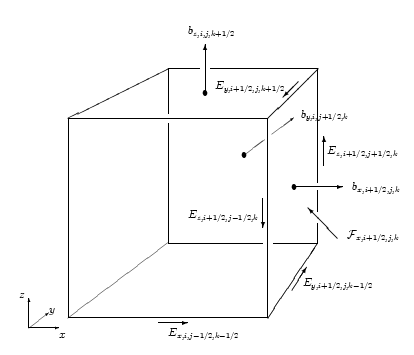
\includegraphics[width=5in]{MHD_GridStaggeredMesh}}
\end{center}
\caption{\label{Fig:GridStaggeredControlVolume3D} A 3D control volume
on the staggered grid with the cell center at $(i,j,k)$. The magnetic
fields are collocated at the cell face centers and the electric fields
at the cell edge centers. The line integral of the electric fields
$\int_{{\partial \mathcal{F}_n}} \mathbf{E}\cdot\mathbf{T}dl$ along
the four edges of the face $\mathcal{F}_{x,i+1/2,j,k}$ gives rise
to the negative of the rate of change of the magnetic field flux
in $x$-direction through the area enclosed by the four edges
(\ie, the area of $\mathcal{F}_{x,i+1/2,j,k}$).}
\end{figure}


\begin{table}
\caption{ Runtime parameters used in 
the unsplit staggered mesh MHD (\code{physics/Hydro/HydroMain/unsplit/MHD\_StaggeredMesh}) solver
additional to those described for the unsplit hydro solver 
(\code{physics/Hydro/HydroMain/unsplit/Hydro\_Unsplit}).}
\label{Tab:mhd usm parameters} 
\begin{center}
\begin{tabular}{lllp{3in}}
Variable & Type  & Default & Description\\
\hline
\code{killdivb}	       & logical & .true.   & On/off $\nabla \cdot \mathbf{B}=0$ handling on the staggered grid\\
\code{E\_modification} & logical & .true.   & Enable/disable high-order electric field construction\\
\code{E\_upwind}       & logical & .false.  & Enable/disable an upwind update for induction equations\\
\code{energyFix}       & logical & .true.   & Enable/disable energy correction\\
\code{facevar2ndOrder} & logical & .true.   & Turn on/off a second-order facevar update \\
\code{ForceHydroLimit} & logical & .false.  & On/off pure Hydro mode\\ 
\code{prolMethod}      & string  & "INJECTION\_PROL" & Use either direct injection method ("INJECTION\_PROL") 
or Balsara's method ("BALSARA\_PROL") in prolonging divergence-free magnetic fields stored in face-centered variables\\
\code{RiemannSolver}   & string  & "ROE"    & "HLLD" is additionally available for MHD, "Hybrid" is also available for MHD.\\
\hline
\end{tabular}
\end{center}
\end{table}

\begin{flashtip}[Stability limit]
As described in the unsplit hydro solver unit (\code{physics/Hydro/HydroMain/unsplit\/Hydro\_Unsplit}), the USM MHD 
solver can take a wide range of CFL limits in all three dimensions (\ie, CFL $<$ 1). 
However, in some circumstances where there are strong shocks and rarefactions, \code{shockLowerCFL=.true.} 
could be useful to gain more numerical
stability by using. It is also helpful to use %(1) using the more stable Donor cell method, and 
(1) artificial viscosity and flattening, or
(2) lower order reconstruction scheme (e.g., MH), or
(2) diffusive Riemann solver such as HLL-type, or LLF solvers, or
(3) a reduced CFL accordingly.
%This approach will automatically revert such reduced 
%stability conditions to any given original condition set by users when there are no significant shocks and rarefactions detected.
\end{flashtip}

\begin{flashtip}[Divergence-free prolongation of magnetic fields on AMR in the unsplit staggered mesh solver]
It is of importance to preserve divergence-free evolutions of magnetic fields in MHD
simulations. Moreover, some special cares are required in prolonging 
divergence-free magnetic fields on AMR grids. One simple straightforward way
in this aspect is to prolong divergence-free fields to newly created children
blocks using direct injection. This injection method therefore inherently 
preserves divergence-free properties on AMR block structures 
and works well in most cases. This method is a default in the unsplit staggered mesh
solver and can also be enabled by setting a runtime parameter
\code{prolMethod = "INJECTION\_PROL"}. Another way, proposed by Balsara (2001), is also
available in the unsplit staggered mesh solver and can be chosen by setting \code{prolMethod = "BALSARA\_PROL"}.
Both prolongation methods are supported in MHD's 2.5D and 3D simulations.
In 2 and 2.5D cylindrical geometry however, since neither method takes into account
geometrical factors, we use a modified prolongation algorithm based on
Balsara (2004) and Li\&Li (2004). This is the default option and is
activated by choosing \code{prolMethod = "BALSARA\_PROL"}.
The need for this special refinement requires to have an MHD's own customized
implementation of \code{Simulation_customizeProlong.F90} placed in the 
\code{source/Simulation/SimulationMain/magnetoHD/}.
% As a known issue, however, Balsara's method works properly only 
% for \Paramesh4.0 but not for \Paramesh4dev in the \flashxtwo release. 
% The direct injection method works for both \Paramesh implementations.
\end{flashtip}
